\documentclass[a4paper, 11pt, titlepage, english]{article}

\usepackage{babel}
\usepackage[utf8]{inputenc}
\usepackage[T1]{fontenc, url}
\usepackage{textcomp}
\usepackage{amsmath, amssymb}
\usepackage{amsbsy, amsfonts}
\usepackage{graphicx, color}
\usepackage{parskip}
\usepackage{framed}
\usepackage{amsmath}
\usepackage{xcolor}
\usepackage{multicol}
\usepackage{url}
\usepackage{flafter}


\usepackage{geometry}
\geometry{headheight=0.01mm}
\geometry{top=24mm, bottom=30mm, left=39mm, right=39mm}

\definecolor{javared}{rgb}{0.6,0,0} % for strings
\definecolor{javagreen}{rgb}{0.25,0.5,0.35} % comments
\definecolor{javapurple}{rgb}{0.5,0,0.35} % keywords
\definecolor{javadocblue}{rgb}{0.25,0.35,0.75} % javadoc

\usepackage{listings}
\lstset{language=python,
basicstyle=\ttfamily\footnotesize,
keywordstyle=\color{javapurple}\bfseries,
stringstyle=\color{javared},
commentstyle=\color{javagreen},
morecomment=[s][\color{javadocblue}]{/**}{*/},
% numbers=left,
% numberstyle=\tiny\color{black},
stepnumber=2,
numbersep=10pt,
tabsize=2,
showspaces=false,
showstringspaces=false,
frame= single,
breaklines=true}

%
% Definering av egne kommandoer og miljøer
%
\newcommand{\dd}[1]{\ \text{d}#1}
\newcommand{\f}[2]{\frac{#1}{#2}} 
\newcommand{\beq}{\begin{equation*}}
\newcommand{\eeq}{\end{equation*}}
\newcommand{\bra}[1]{\langle #1|}
\newcommand{\ket}[1]{|#1 \rangle}
\newcommand{\braket}[2]{\langle #1 | #2 \rangle}
\newcommand{\braup}[1]{\langle #1 \left|\uparrow\rangle\right.}
\newcommand{\bradown}[1]{\langle #1 \left|\downarrow\rangle\right.}
\newcommand{\av}[1]{\left| #1 \right|}
\newcommand{\op}[1]{\hat{#1}}
\newcommand{\braopket}[3]{\langle #1 | {#2} | #3 \rangle}
\newcommand{\ketbra}[2]{\ket{#1}\bra{#2}}
\newcommand{\pp}[1]{\frac{\partial}{\partial #1}}
\newcommand{\ppn}[1]{\frac{\partial^2}{\partial #1^2}}
\newcommand{\up}{\left|\uparrow\rangle\right.}
\newcommand{\upup}{\left|\uparrow\uparrow\rangle\right.}
\newcommand{\down}{\left|\downarrow\rangle\right.}
\newcommand{\downdown}{\left|\downarrow\downarrow\rangle\right.}
\newcommand{\updown}{\left|\uparrow\downarrow\rangle\right.}
\newcommand{\downup}{\left|\downarrow\uparrow\rangle\right.}
\newcommand{\bupup}{\left.\langle\uparrow\uparrow\right|}
\newcommand{\bdowndown}{\left.\langle\downarrow\downarrow\right|}
\newcommand{\bupdown}{\left.\langle\uparrow\downarrow\right|}
\newcommand{\bdownup}{\left.\langle\downarrow\uparrow\right|}
\renewcommand{\d}{{\rm d}}

\newcommand{\To}{\quad \Rightarrow\quad}



\renewcommand{\arraystretch}{1.6}
\setlength{\tabcolsep}{10pt}
\makeatletter
\renewcommand*\env@matrix[1][*\c@MaxMatrixCols c]{%
  \hskip -\arraycolsep
  \let\@ifnextchar\new@ifnextchar
  \array{#1}}
\makeatother

%
% navn og tittel
%
\author{Jonas van den Brink}
\title{Problem set 1 \\ FYS3140}


\begin{document}

\section*{Oppgave 1}
Vi antar at vi har stokastiske variable $X_1$, $X_2$, $\ldots$, $X_n$, som er er uavhengige og uniformt fordelt på intervallet $[0,\theta]$, dvs at de har tetthet
$$f(x; \theta) = \begin{cases}
                  1/\theta & \mbox{for } 0 \leq x \leq \theta, \\
                  0 & \mbox{ellers}.
                 \end{cases}$$
Parameteren $\theta$ er ukjent, og skal estimeres.
\subsection*{a)}
Vi starter med å finne forventingen av $X_i$, som per definisjon gitt ved
$$E(X_i) = \int_{-\infty}^\infty x f(x; \theta) \ \d x,$$
setter inn uttrykket for sannsynlighetsfordelingen og ser at bare $x\in(0,\theta]$ gir bidrag til integralet:
$$E(X_i) = \int_0^\theta \frac{x}{\theta} \ \d x = \frac{\theta^2}{2\theta} = \frac{\theta}{2}.$$

Vi kan finne variansen til $X_i$ fra uttrykket
$$V(X_i) = E(X_i^2) - E(X_i)^2,$$
vi må da først finne $E(X_i^2)$, som gjøres likt som tidligere:
$$E(X_i^2) = \int_{-\infty}^\infty x^2 f(x; \theta) \ \d x = \int_0^\theta \frac{x^2}{\theta} \ \d x = \frac{\theta^2}{3}.$$
Variansen er da
\begin{align*}
V(X_i) = E(X_i^2) - E(X_i)^2 = \frac{\theta^2}{12}.
\end{align*}

Vi har altså vist følgende
$$E(X_i) = \frac{\theta}{2}, \qquad V(X_i) = \frac{\theta^2}{12}.$$

\subsection*{b)}
Vi finner momentestimatoren for $\theta$ ved å sette det første distribusjonsmomentet, $E(X_i)$, lik det første samplingsmomentet, $\overline{X}$
$$E(X_i) = \frac{1}{n}\sum_{i=1}^n X_i,$$
vi setter inn for forventningen og løser for estimatoren
$$\frac{\hat{\theta}_{\rm mom}}{2} = \overline{X} \To \hat{\theta}_{\rm mom} = 2\overline{X}.$$

Forventningen av momentestimatoren blir
$$E(\hat{\theta}_{\rm mom}) = E(2\overline{X}),$$
setter inn for $\overline{X}$ og bruker linearitet av forventningen
\begin{align*}
E(\hat{\theta}_{\rm mom}) &= E\bigg(\frac{2}{n}\sum_{i=1}^n X_i\bigg) = \frac{2}{n}\sum_{i=1}^n E(X_i) = \frac{2}{n}\frac{n\theta}{2} =  \theta.
\end{align*}
Ettersom at 
$$E(\hat{\theta}_{\rm mom}) - \theta = 0,$$
ser vi at momentestimatoren er en forventningsrett estimator.

\subsection*{c)}
Standardfeilen til momentestimatoren er gitt ved
$$\sigma_{\hat{\theta}_{\rm mom}} = \sqrt{V(\hat{\theta}_{\rm mom})},$$
vi finner derfor først variansen til estimatoren, bruker da at vi generelt for variansen har
$$V\bigg(a + \sum_i b_i X_i\bigg) = \sum_i b_i^2 V(X_i).$$
Finner at
$$V(\hat{\theta}_{\rm mom}) = V\bigg(\sum_{i=1}^n \frac{2}{n} X_i\bigg) = \frac{4}{n^2}\sum_{i=1}^n V(X_i) = \frac{4}{n^2}\frac{n\theta^2}{12} = \frac{\theta^2}{3n}.$$
Slik at standardfeilen blir
$$\sigma_{\hat{\theta}_{\rm mom}} = \frac{\theta}{\sqrt{3n}}.$$

Vi kan nå vise at estimatoren er konsistent ved å bruke Chebychevs ulikhet, som sier at for enhver stokastisk variabel $X$, med forventning $\mu$ og varians $\sigma^2$, så vil
$$P(|X-\mu| > t) \leq \frac{\sigma^2}{t^2},$$
gjelde for alle $t > 0$. Momentestimatoren $\hat{\theta}_{\rm mom}$ er en stokastisk variabel med forventning $\mu=\theta$ og varians $\sigma^2 = \theta^2/3n$, vi setter dette inn i ulikheten og får
$$P(|\hat{\theta}_{\rm mom} - \theta| > t) \leq \frac{\theta^2}{3nt^2}.$$
Vi ser at for en hvilken $t > 0$ vi velger, kan vi gjøre uttrykket på høyre side mindre enn en hvilken som helst tolerans $\epsilon > 0$ ved å velge $n > N$ for en eller annen $N$. Det vil si at momentestimatoren konvergerer mot $\theta$ i sannsynlighet når $n$ vokser.

\subsection*{d)}
Siden de stokastiske variable $X_1$, $X_2$, $\ldots$ $X_n$ er uavhengige, så vil likelihooden være produktet av de individuelle sannsynlighetsfordelingene
$$f(x_1, x_2, \ldots, x_n; \theta) = \prod_{i=1}^n f(x_i; \theta).$$
Ved å sette inn $f(x_i; \theta)$ ser vi at produktet blir 
$$
f(x_1, x_2, \ldots, x_n; \theta) = \begin{cases}
                                      \big(1/\theta)^n & \mbox{ for } 0 \leq x_1, \ldots, x_n \leq \theta\\
                                      0 & \mbox { ellers.}
                                     \end{cases}.
$$

\subsection*{e)}
Vi skal nå finne maksimum likelihood estimatoren $\hat{\theta}_{\rm max}$, det vil si den verdien av den ukjente parameteren $\theta$ slik at likelihooden er maksimert: 
$$f(x_1, x_2, \ldots, x_n; \hat{\theta}_{\rm max}) \geq f(x_1, x_2, \ldots, x_n; \theta).$$ 
Vi er altså ute etter å finne et globalt maksimum i likelihood funksjon
$$
f(x_1, x_2, \ldots, x_n; \theta) = \begin{cases}
                                      \big(1/\theta)^n & \mbox{ for } 0 \leq x_1, \ldots, x_n \leq \theta\\
                                      0 & \mbox { ellers.}
                                     \end{cases}.
$$
Vi ser med en gang at en mindre $\theta$ betyr en større sannsynlighet, så lenge ikke $\theta < x_1, x_2, \ldots, x_n$, vi lar derfor 
$$\hat{\theta}_{\rm max} = \max_{1\leq i\leq n} X_i.$$
Merk at vi ikke kan finne dette maksimumet ved å derivere likelihood-funksjonen fordi likelihood funksjonen har en diskontinuitet akkurat i dette punktet.

\subsection*{f)}
Sannsynlighetstettheten til den største sampelen fra en stokastisk variabel med sannsynlighetstetthet $f(x)$ og kumulativ sannsynlighet $F(x)$  er gitt ved\footnote{Se \emph{Devore} \& \emph{Berk} avsnitt 5.5, side 268-269}
$$g_n(y) = n\big[F(y)\big]^{n-1} \cdot f(y).$$
Vi vet at for $X_i$ har vi tettheten
$$f(x; \theta) = \begin{cases}
                  1/\theta & \mbox{for } 0 \leq x \leq \theta, \\
                  0 & \mbox{ellers},
                 \end{cases}$$
slik at den kumulative sannsynligheten blir
$$F(x; \theta) = \begin{cases}
		  0 & \mbox{ for } x < 0 \\
		  \int_0^x  \frac{1}{\theta} \ \d x' = \frac{x}{\theta} & \mbox{ for } 0 \leq x \leq \theta \\
		  1 & \mbox{ for } x > \theta,
                 \end{cases}
                 $$
$$\int_0^x  \frac{1}{\theta} \ \d x' = \frac{x}{\theta}.$$
Innsetting gir da at sannsynlighetstettheten til maksimum likelihood estimatoren er
$$g_n(y) = n\bigg(\frac{y}{\theta}\bigg)^{n-1} \frac{1}{\theta} = \frac{ny^{n-1}}{\theta^n}.$$ 

\subsection*{g)}
Ettersom at vi nå kjenner sannsynlighetsfordelingen til maksimum likelihood estimatoren, kan vi finne forventningen til estimatoren direkte
$$E(\hat{\theta}_{\rm max}) = \int_{-\infty}^{\infty} y \cdot g_n(y) \ \d y,$$
innsetting gir
$$E(\hat{\theta}_{\rm max}) = \int_0^\theta \frac{nx^n}{\theta^n} \ \d y = \frac{n}{n+1}\theta.$$

\subsection*{h)}
Vi ser fra forventningen til maksimums likelihood estimatoren at den ikke er forventningsrett. Ettersom at forventningen er lineær, ser vi at vi kan lage en forventningsrett estimator ved å gange inn en faktor:
$$\hat{\theta}_{\rm mod} = \frac{n+1}{n}\hat{\theta}_{\rm max},$$
slik at vi har
$$E(\hat{\theta}_{\rm mod}) = E\bigg(\frac{n+1}{n}\hat{\theta}_{\rm max}\bigg) = \frac{n+1}{n} E(\hat{\theta}_{\rm max}) = \frac{n+1}{n}\frac{n}{n+1}\theta = \theta.$$

Standardfeilen til den modifiserte estimatoren blir
$$\sigma_{\hat{\theta}_{\rm mod}} = \sqrt{V(\hat{\theta}_{\rm mod})},$$
der variansen er
$$V(\hat{\theta}_{\rm mod}) = V\bigg(\frac{n+1}{n}\hat{\theta}_{\rm max}\bigg) = \frac{(n+1)^2}{n^2}V(\hat{\theta}_{\rm max}).$$
Variansen til maksimums likelihood estimatoren er igjen
$$V(\hat{\theta}_{\rm max}) = E(\hat{\theta}_{\rm max}^2) - E(\hat{\theta}_{\rm max})^2,$$
der 
$$E(\hat{\theta}_{\rm max}) = \frac{n}{n+1}\theta,$$
og 
$$E(\hat{\theta}_{\rm max}^2) = \int_0^\theta \frac{nx^{n+1}}{\theta^n} \ \d x = \frac{n}{n+2}\theta^2.$$

Innsetting gir da
$$V(\hat{\theta}_{\rm mod}) = \frac{(n+1)^2}{n^2} \bigg(\frac{n}{n+2}\theta^2 - \frac{n^2}{(n+1)^2}\theta^2\bigg),$$
som videre gir 
$$V(\hat{\theta}_{\rm mod}) = \frac{n^2+2n+1 - n^2 - 2n}{n(n+2)}\theta = \frac{\theta^2}{n(n+2)}.$$
Slik at standardfeilen er
$$\sigma_{\hat{\theta}_{\rm mod}} = \frac{\theta}{\sqrt{n(n+2)}}.$$

\subsection*{i)}
Vi har nå funnet to forventningsrette estimatorer:
$$\hat{\theta}_{\rm mom} = 2\overline{X}, \qquad \hat{\theta}_{\rm mod} = \frac{n+1}{n}\bigg(\max_{1\leq i\leq n} X_i\bigg).$$
Med standardfeilene
$$\sigma_{\hat{\theta}_{\rm mom}} = \frac{\theta}{\sqrt{3n}}, \qquad \sigma_{\hat{\theta}_{\rm mod}} = \frac{\theta}{\sqrt{n(n+2)}}.$$
Vi ser nå at selv om begge estimatorene konvergerer mot $\theta$ med økende $n$, så går momentestimatoren som $\mathcal{O}(1/\sqrt{n})$, mens den modifiserte estimatoren går som $\mathcal{O}(1/n)$. Den modifiserte estimatoren har altså en mye bedre asymptotisk oppførsel en momentestimatoren, om vi har mulighet til å ta mange samples er det altså den modifiserte estimatoren som er å foretrekke.

\subsection*{j)}
Vi skal nå gjennomføre et numerisk eksperiment for å teste resultatet vi har funnet. Vi trekker $n=20$ samples fra en uniform fordeling med parameter $\theta=1$, vi regner så ut hva de to estimatorene estimerer at $\theta$ faktisk er, vi gjør dette 1000 ganger på rad og lager et histogram av resultatene. For å undersøke den asymptotiske oppførselen til de to estimatoren gjentar vi forsøket for $n=200$ og $n=2000$. Se vedlegg 1 for kildekoden og figur \ref{fig:hist}, \ref{fig:hist2} og \ref{fig:hist3} for resultatene. 

Vi ser at den modifiserte estimatoren har en mye skarpere topp og ligger generelt sett nærmere den faktiske verdien av $\theta$ enn det momentestimatoren gjør, og vi ser at dette bare blir klarere når $n$ økes, slik som vi har kommet frem til. Vi ser også at momentestimatoren legger seg ganske symmetrisk om $\theta$, mens den modifiserte estimatoren derimot er asymmetrisk og har mer tendens til å legge seg under $\theta$.

\begin{figure}
\centering
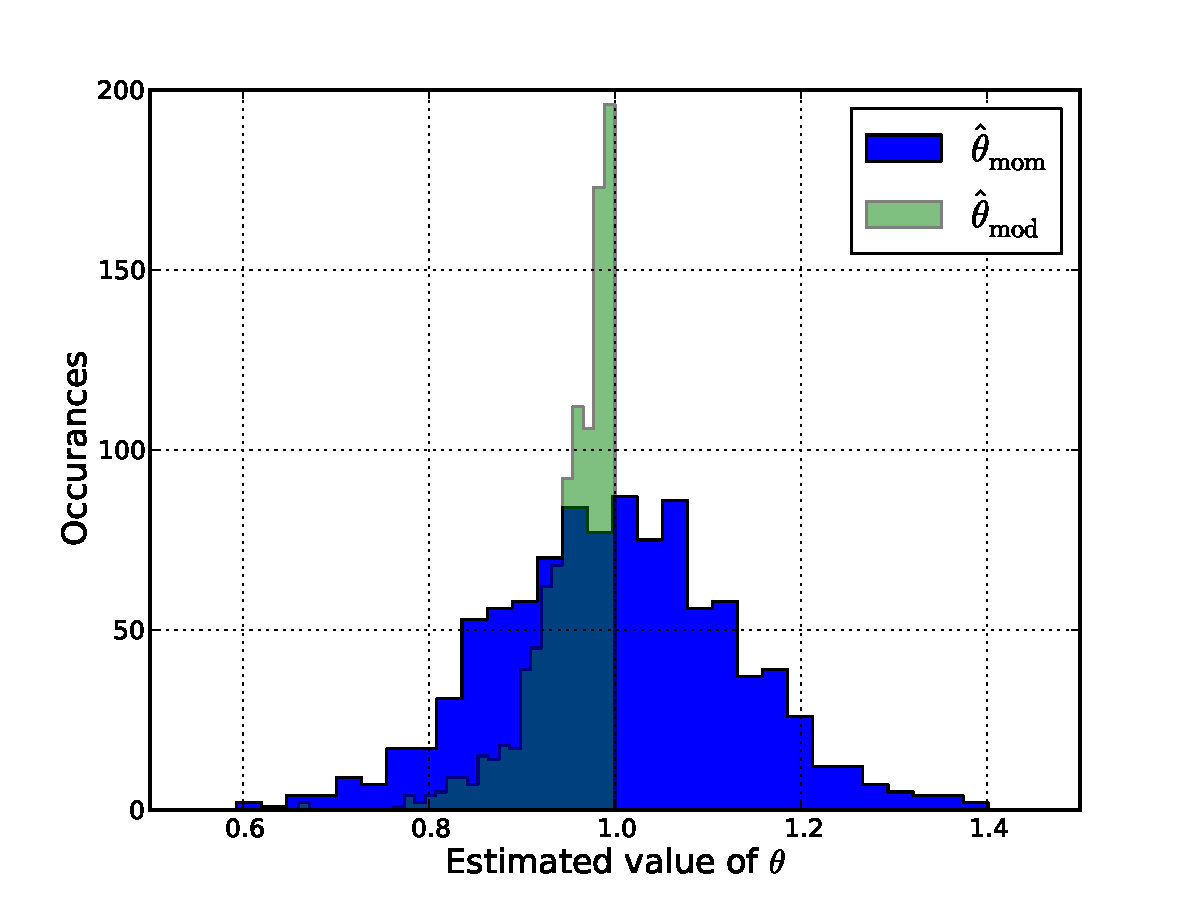
\includegraphics[width=\textwidth]{estimators_hist_n20.pdf}
\caption{Resultatene av $N=1000$ forsøk med $n=20$ samples hver presentert i et histogram. \label{fig:hist}}
\end{figure}

\begin{figure}
\centering
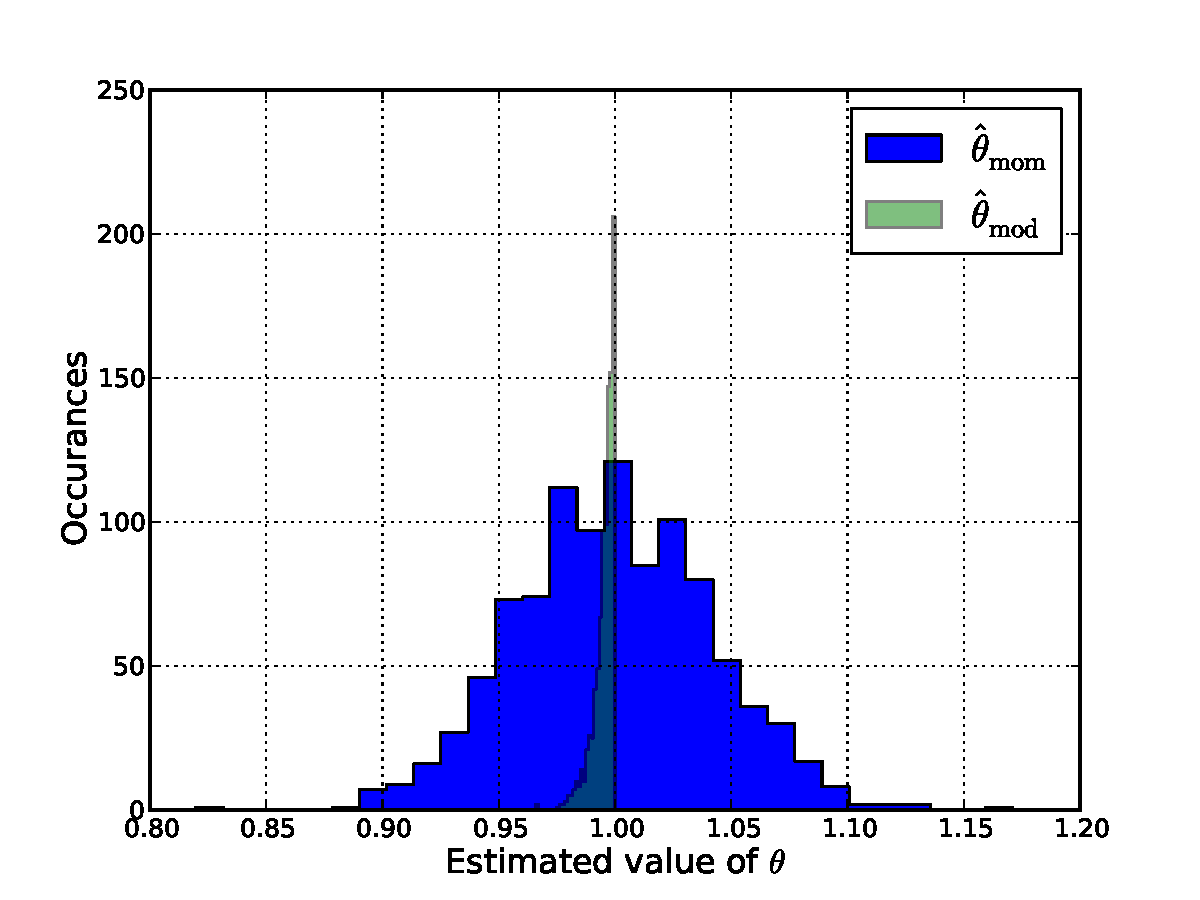
\includegraphics[width=\textwidth]{estimators_hist_n200.pdf}
\caption{Resultatene av $N=1000$ forsøk med $n=200$ samples hver presentert i et histogram. \label{fig:hist2}}
\end{figure}

\begin{figure}[t]
\centering
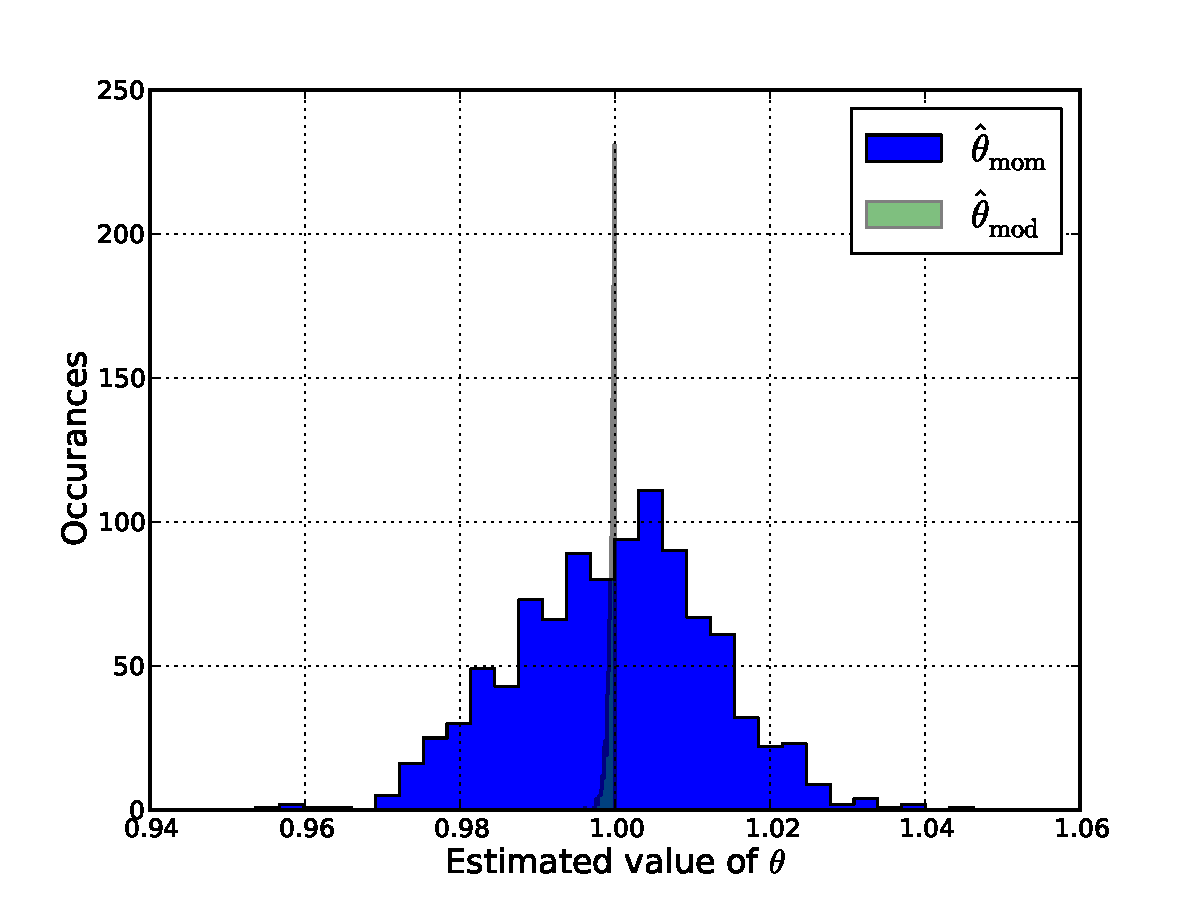
\includegraphics[width=\textwidth]{estimators_hist_n2000.pdf}
\caption{Resultatene av $N=1000$ forsøk med $n=2000$ samples hver presentert i et histogram. \label{fig:hist3}}
\end{figure}

\clearpage



\section*{Problem 2}
\subsection*{a)}
Ettersom at vi ikke kjenner det faktiske standardavviket $\sigma$, bruker vi istedet det empiriske standardavviket $S$, vi finner derfor først $\overline{X}$ og $S$:
$$\overline{X} = 14.36, \quad S  = \sqrt{\frac{\sum_i (x_i - \overline{x})^2}{n-1}} = 1.156.$$
Et 95\% konfidensintervall for forventningen $\mu$ kan da finnes fra
$$P\bigg(-1.96 < \frac{\overline{X} - \mu}{S/\sqrt{n}}< 1.96 \bigg) \approx 0.95.$$
Vi manipulerer ulikheten og finner at
$$\overline{X} - \frac{1.96S}{\sqrt{n}} < \mu < \overline{X} + \frac{1.96S}{\sqrt{n}}.$$
Slik at konfidensintervallet er
$$\overline{X} \pm \frac{1.96S}{\sqrt{n}}.$$
Ved innsett av verdier finner vi at et 95\% konfidensintervall for $\mu$ er
$$(13.76, 14.97).$$

\clearpage

\subsection*{b)}
Vi skal nå gjennomføre et numerisk eksperiment hvor vi genererer $N=1000$ datasett, hvert av størrelse $n=14$ observasjoner. Vi lar de 14 stokastiske variable være uavhengige og normalfordelt med parametere $\mu = 14.5$ og $\sigma=1$. For hvert av datasettene regner vi ut et 95 \% konfidensintervall, merk at vi i dette tilfelle kjenner standardavviket $\sigma$, så vi slipper å gå veien om det empirsike standardavviket $S$. Etter å ha generert de 1000 datasettene og tilhørende konfidensintervall, teller vi opp antallet av intervallene som inneholder den faktiske verdien av $\mu$. Koden er lagt ved som vedlegg 2 på slutten av oppgaven.

Vi kjører programmet vårt 100 ganger, og lager et histogram av resultatene, ser figur \ref{fig:2b}. Vi ser fra resultatene at $\mu$ er inneholdt i konfidensintervallet ca. 95 \% av datasettene. Vi legger samtidig merke til at dette langt ifra alltid er nøyaktig 95 \%, og at hvor mange ganger $\mu$ ligger innenfor konfidensintervallet er en stokastisk variabel.

\begin{figure}[htpb]
\centering
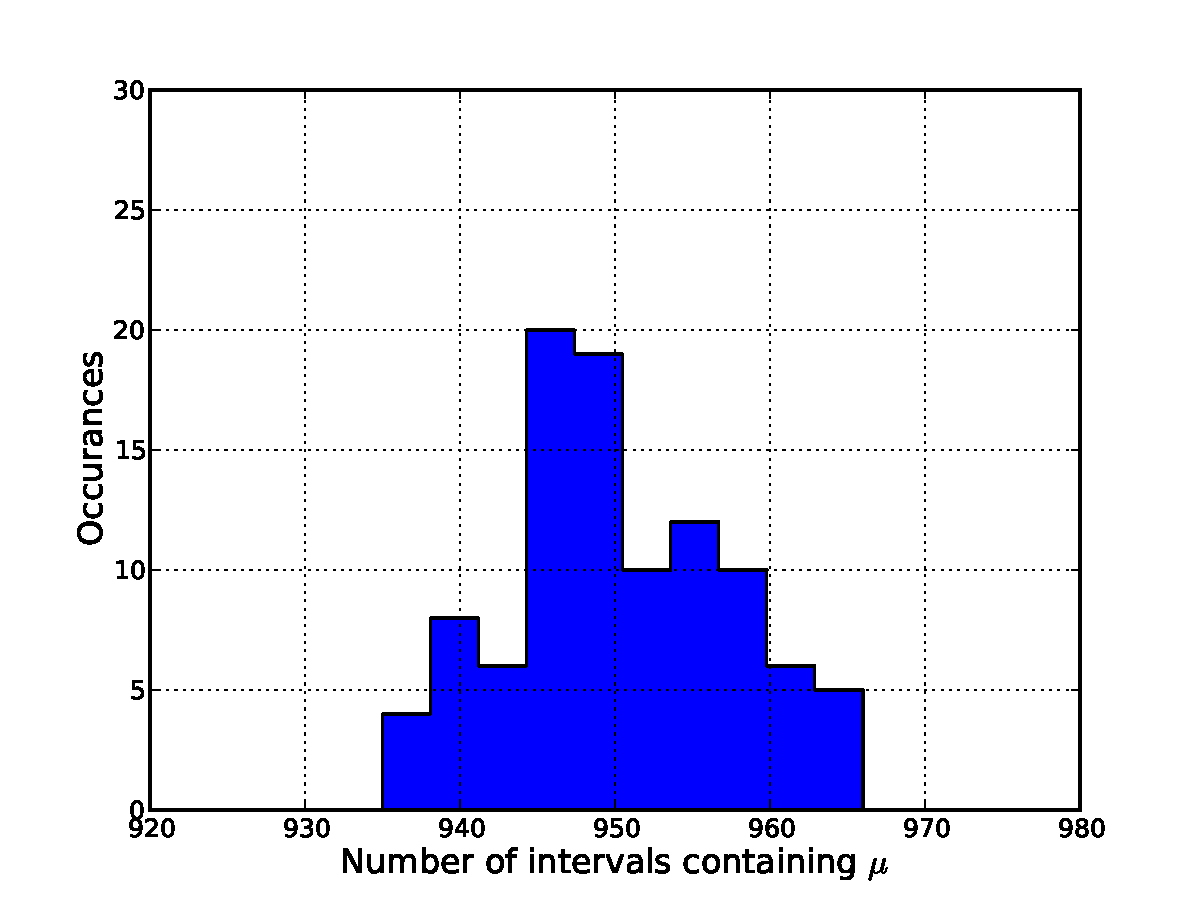
\includegraphics[width=\textwidth]{2b.pdf}
\caption{Resultatene av 100 forsøk med 1000 datasett hver. \label{fig:2b}}
\end{figure}

\clearpage

\subsection*{c)}
Vi gjennomfører nå akkurat det samme eksperimentet, men bruker nå det empiriske standardavviket $S$ istedetfor den faktiske variansen $\sigma$. Vi gjennomfører igjen 100 forsøk og plotter resultatene i figur \ref{fig:2c}.

Vi ser igjen at antall intervaller som inneholder $\mu$ er en stokastisk variabel. I dette tilfellet ser derimot ikke lenger histogrammet ut til å være sentrert rundt $950$, eller 95 \%, forekomster, men mer mot 93 \%. Denne lille forskjellen skyldes at vi ikke bruker vår kunnskap om standardavviket $\sigma$, men må isteden bruke det empiriske standardavviket, som da innfører litt mer usikkerthet.

\begin{figure}[htpb]
\centering
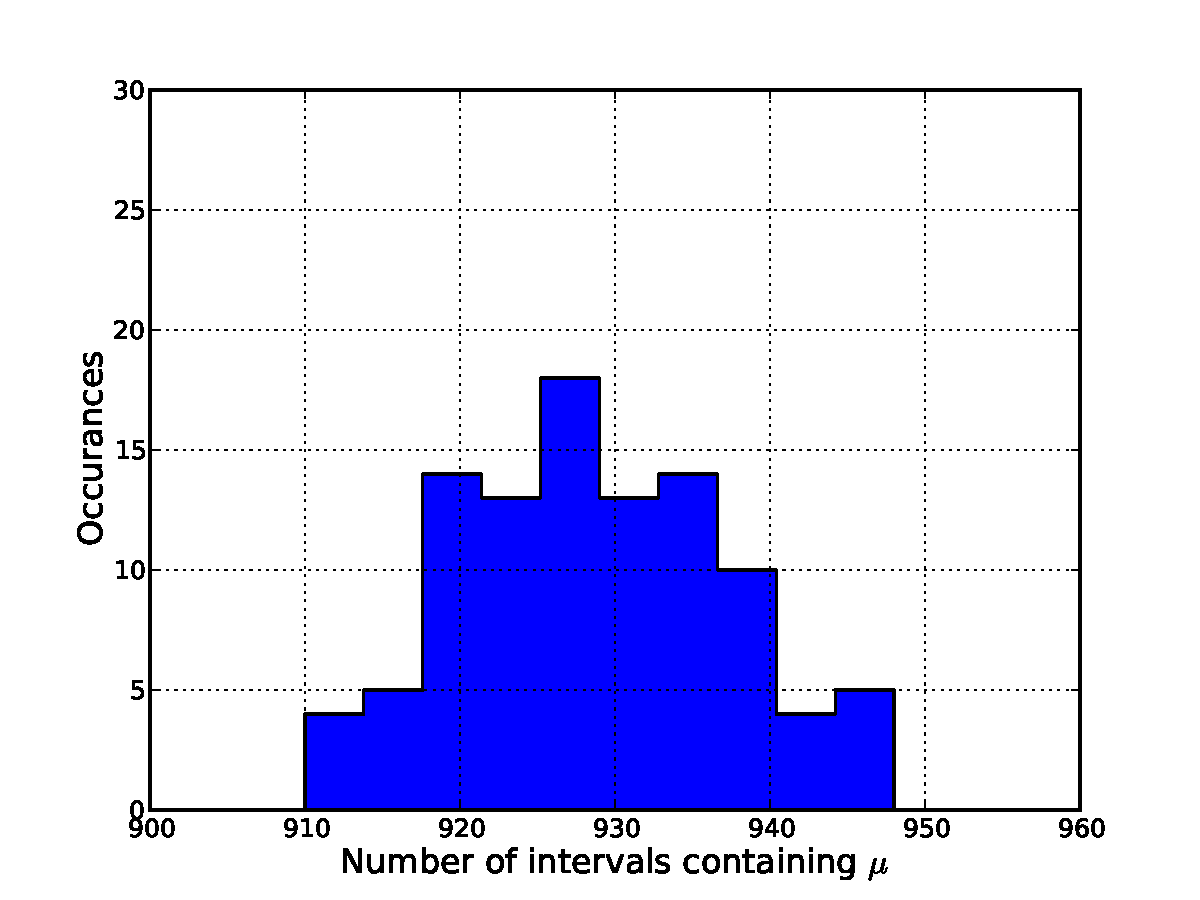
\includegraphics[width=\textwidth]{2c.pdf}
\caption{Resultatene av 100 forsøk med 1000 datasett hver. \label{fig:2c}}
\end{figure}

\subsection*{d)}
Som vi har påpekt tidligere, er antallet av konfidensintervallene som faktisk inneholder $\mu$ en stokastisk variabel. Denne stokastiske variabelen vil ha en binomisk fordeling, ettersom at det for hvert intervall er en sannsynlighet $p$ for at $\mu$ er inneholdt, og en sannsynlighet $1-p$ for at $\mu$ ikke er inneholdt. Ettersom at $p$ er lik for alle datasettene vil resultatet være binomisk fordelt.

\clearpage

\subsection*{e)}
Vi skal nå vise at $13\cdot S^2/\sigma^2$ er $\chi^2$-fordelt med 13 frihetsgrader. Vi starter med å bevise et lemma som viser hvordan differansen av to $\chi^2$-fordelte variabler er fordelt.

\noindent\makebox[\linewidth]{\rule{\textwidth}{0.4pt}}
\paragraph{Lemma:} Hvis $X_3 = X_1 + X_2$, der $X_1\sim\chi_{\nu_1}^2$, $X_3\sim\chi_{\nu_3}^2$, der $\nu_3 > \nu_1$, og $X_1$ og $X_2$ er uavhengige, da er $X_2 \sim \chi^2_{\nu_3 - \nu_1}$.

\paragraph{Bevis:} Ettersom at $X_1$ og $X_2$ er uavhengige, så vil den momentgenererende funksjonen til $X_3$ være gitt ved produktet av de momentgenererende funksjonene til $X_1$ og $X_2$, slik at
$$M_{X_3}(t) = M_{X_1 + X_2}(t) = M_{X_1}(t)M_{X_2}(t).$$
Vi vet samtidig at den momentgenererende funksjonen for en $\chi^2$-fordelt variabel med $\nu$ frihetsgrader er $(1-2t)^{-\nu/2}$. slik at
$$(1-2t)^{-\nu_3/2} = (1-2t)^{-\nu_1/2}M_{X_2}(t).$$
Vi løser nå for $M_{X_2}(t)$:
$$M_{X_2}(t) = (1-2t)^{-(\nu_3 - \nu_1)/2},$$
og ettersom at $\nu_3 > \nu_1$ ser vi at dette svarer til den momentgenererende funksjonen til en $\chi^2$-fordelt variabel med $\nu_3 - \nu_1$ frihetsgrader. Siden momentgenererende funksjoner er entydige, må altså $X_2 \sim \chi^2_{\nu_3-\nu_1}$.

\noindent\makebox[\linewidth]{\rule{\textwidth}{0.4pt}}

Vi starter nå med å definere en stokastisk variabel $X_3$ som følger:
$$X_3 = \sum_{i=1}^{14} \bigg(\frac{X_i - \mu}{\sigma}\bigg)^2.$$
Vi vet nå at $X_3\sim\chi^2_{14}$, fordi $X_3$ er summen av 14 kvadrerte standardnormalfordelte variable. Vi utvider nå innsiden av summen ved å legge til og trekke fra $\overline{X}$
$$X_3 = \sum_{i=1}^{14} \bigg(\frac{X_i - \overline{X}}{\sigma} + \frac{\overline{X} - \mu}{\sigma}\bigg)^2,$$
vi ganger ut og finner
$$X_3 =  \sum_{i=1}^{14} \bigg(\frac{X_i - \overline{X}}{\sigma}\bigg)^2 + \sum_{i=1}^{14} 2\bigg(\frac{X_i - \overline{X}}{\sigma}\bigg)\bigg(\frac{\overline{X} - \mu}{\sigma}\bigg) +\sum_{i=1}^{14} \bigg(\frac{\overline{X} - \mu}{\sigma}\bigg)^2$$
Den midterste summen blir null, fordi
$$ \sum_{i=1}^{14} 2\bigg(\frac{X_i - \overline{X}}{\sigma}\bigg)\bigg(\frac{\overline{X} - \mu}{\sigma}\bigg) = 2 \bigg(\frac{\overline{X} - \mu}{\sigma^2}\bigg)\sum_{i=1}^{14} \big(X_i - \overline{X}\big) = 0.$$
Mens den siste summen avhenger ikke av $i$, slik at vi har
$$X_3 =  \sum_{i=1}^{14} \bigg(\frac{X_i - \overline{X}}{\sigma}\bigg)^2 + 14\bigg(\frac{\overline{X} - \mu}{\sigma}\bigg)^2.$$
som kan skrives om til
$$X_3 =  \sum_{i=1}^{14} \bigg(\frac{X_i - \overline{X}}{\sigma}\bigg)^2 + \bigg(\frac{\overline{X} - \mu}{\sigma/\sqrt{14}}\bigg)^2.$$
Vi gjenkjenner det første leddet på venstre side som $13\cdot S^2/\sigma^2$, og det siste leddet som en standardnormalfordeltvariabel kvadrert, slik at
$$X_3 = 13\cdot S^2/\sigma^2 + X_1, \mbox{ der } X_1 \equiv \bigg(\frac{\overline{X} - \mu}{\sigma/\sqrt{14}}\bigg)^2.$$
Vi vet nå at $X_3 \sim \chi^2_{14}$ og $X_1\sim \chi^2_1$, men før vi kan si med sikkerhet at $13\cdot S^2/\sigma^2 \sim \chi^2_{14-1}$ må vi vise at $13\cdot S^2/\sigma^2$ og $X_1$ er uavhengige. Vi ser at $13\cdot S^2/\sigma^2$ bare avhenger av den stokastiske variabelen $S^2$, mens $X_1$ avhenger av $\overline{X}$, og vi vet fra før at $S^2$ og $\overline{X}$ er uavhengige. Så da har vi vist at
$$X_2 = 13\cdot S^2/\sigma^2 \sim \chi^2_{13}.$$


\subsection*{f)}
Vi vil nå beregne et 99\% konfidensintervall for $\sigma^2$. Vi har vist at $13\cdot S^2/\sigma^2 \sim \chi^2_{13}$, slik at vi vet\footnote{Se \emph{Devore} \& \emph{Berk} tabell A.7, side 791.}
$$P(3.565\leq13\frac{S^2}{\sigma^2}\leq 29.817) = 0.99.$$
Vi løser ulikheten
$$3.565\leq13\frac{S^2}{\sigma^2}\leq 29.817,$$
for $\sigma^2$ ved å ta resiproken, og finner
$$\frac{13S^2}{3.565} \geq \sigma^2 \geq \frac{13S^2}{29.817},$$
setter vi inn for $S^2 = 1.336$ (se oppg 2a), finner vi at et 99\% konfidensintervall for $\sigma^2$ er
$$\sigma^2 \in [0.436, 4.872].$$




\clearpage

\section*{Oppgave 3}

Vi lar nå $X$ være antall tilfeller av en sjelden medfødt sykdom i året, og antar at $X$ er Poisson-fordelt med parameter $\lambda$, slik at
$$P(X = k) = \frac{\lambda^k}{k!}e^{-\lambda}, \mbox{ der } k=0,1,2,\ldots$$

\subsection*{a)}
Parameteren $\lambda$ har vært 1, slik at $H_0:\lambda = 1$, vi skal nå undersøke hvor mange tilfeller man må observere et gitt år for å forkaste $H_0$ til fordel for $H_a: \lambda > 1$ på et nivå $\alpha = 0.05$.

Størrelsen $\alpha$ beskriver sannsynligheten for å gjøre en type I feil, det vil si at vi forkaster $H_0$ selv om den stemmer. For å finne denne sannsynligheten tenker vi oss altså at vi forkaster $H_0$ hvis det er $k$ eller flere tilfeller av sykdommen et gitt år. Ettersom at parameteren er $\lambda = 1$, kan vi lett regne oss frem til sannsynligheten for en type I feil for hver mulig verdi for $k$:
\begin{align*}
\alpha &= P(\mbox{type I error}) \\
&= P(X\geq k) \\
&= 1 - \sum_{i=0}^{k-1} P(X=i) \\
&= 1 - \sum_{i=0}^{k-1} \frac{1}{ek!}.
\end{align*}
Vi har da at
\begin{center}
\begin{tabular}{c|c}
$k$ & $\alpha$ \\
\hline
0 & 1.00 \\
1 & 0.63 \\
2 & 0.26 \\
3 & 0.08 \\
4 & 0.02 
\end{tabular}
\end{center}
Slik at om man vil ha en $\alpha \leq 0.05$, må man velge å forkaste $H_0$ om man observerer minst $k=4$ tilfeller av sykdommen et gitt år.

\clearpage

\subsection*{b)}
Vi fant i forrige oppgave at vi skulle observere minst $k=4$ tilfeller før man forkastet $H_0$, vi antar nå at parameteren faktisk har forandret seg, slik at $\lambda = 2$, og ønsker å finne $\beta$, som er sannsynligheten for en type II feil, det vil si at vi holder på $H_0$ når den faktisk er falsk.
\begin{align*}
\beta &= P(\mbox{type II error}) \\
&= P(X\leq3; \lambda=2) \\
&= \sum_{i=0}^3 P(X=i; \lambda=2)\\
&= \frac{2^0}{0!}e^{-2} + \frac{2^1}{1!}e^{-2} + \frac{2^2}{2!}e^{-2} + \frac{2^3}{3!}e^{-2}\\
&= 0.812.
\end{align*}
Så vi ser at sannsynligheten for en type II feil er mye større en en type I feil i dette tilfellet.

\subsection*{c)}
Lar nå $p$ være sannsynligheten for at et barn blir født med sykdommen. Vi observerer $n_i$ fødte barn og $X_i$ antall tilfeller for hvert år $i$, der $i=1,\ldots,m$. Antar at antall tilfeller hvert år er uavhengige og Poisson-fordelt $X_i \sim \mbox{Poisson}(n_ip), i = 1,\ldots,m$ og skal finn sannsynlighetsmaksimering-estimatoren for sannsynligheten $p$.

Ettersom at antall tilfeller hvert år er uavhengig er likelihood-funksjonen:
$$f(x_1, x_2, \ldots, x_m; p) = \prod_{i=1}^m \frac{(n_ip)^{x_i}}{x_i!}e^{-n_i p}.$$
Tar logaritmen og får
$$\ln[f] = \sum_{i=1}^m \bigg(x_i \ln n_i p - \ln x_i! - n_i p\bigg).$$
Deriverer med hensyn på $p$ og setter lik 0 for å finne maksimummet
$$\frac{\d \ln[f]}{\d p} = \sum_{i=1}^m \frac{\d}{\d p}\bigg(x_i \ln n_i p - \ln x_i! - n_i p\bigg) = 0,$$
som blir
$$\sum_{i=1}^m \bigg(\frac{x_i}{p}  - n_i \bigg) = 0,$$
Vi løser nå for $p$, 
$$\hat{p} = \frac{\sum_i X_i}{\sum_i n_i},$$
vi kan nå utvide brøken med $1/m$, slik at estimatoren er forholdet av gjennomsnittene
$$\hat{p} = \frac{\overline{X}}{\overline{n}},$$

\clearpage

\subsection*{d)}
Vi finner nå forventningen og variansen til estimatoren.

Forventningen blir
\begin{align*}
E(\hat{p}) &= E\bigg(\frac{\overline{X}}{\bar{n}}\bigg) \\
&= \frac{1}{\sum_i n_i}E\bigg(\sum_{i=1}^m X_i\bigg) \\
&= \frac{1}{\sum_i n_i}\sum_{i=1}^m E(X_i) \\
&= \frac{1}{\sum_i n_i}\sum_{i=1}^m n_i p \\
&= \frac{\sum_i n_i}{\sum_i n_i} p \\
&= p.
\end{align*}
Så vi ser at estimatoren er forventningsrett.

Variansen blir
\begin{align*}
V(\hat{p}) &= V\bigg(\frac{\sum_i X_i}{\sum_i n_i}\bigg) \\
&= \bigg(\frac{1}{\sum_i n_i}\bigg)^2\sum_{i=1}^m V(X_i) \\
&= \bigg(\frac{1}{\sum_i n_i}\bigg)^2\sum_{i=1}^m n_i p \\
&= \frac{p}{\sum_i n_i}.
\end{align*}
Så vi ser at variansen avtar når den totale summen av barn født over de $m$ årene øker.

\clearpage

\section*{Vedlegg 1 - Kildekode til oppgave 1j}
\lstinputlisting{estimate.py}

\clearpage

\section*{Vedlegg 2 - Kildekode til oppgave 2b og 2c}
\lstinputlisting{2c.py}

\end{document}

